\section{Modifying and applying Grad-CAM}
\nblink{brats/07\_gradcam.ipynb}

TODO: a pixel is just a class

\subsection{Results}

\begin{figure}[H]
    \centering
    \begin{subfigure}{.33\textwidth}
        \centering
        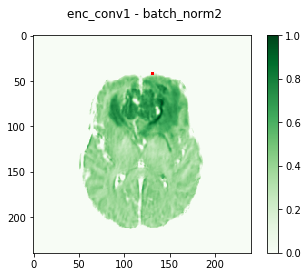
\includegraphics[width=\linewidth]{chapters/04_segmentation/images/grad_cam_03.png}
        \caption{ the text for a}
    \end{subfigure}%
    \begin{subfigure}{.33\textwidth}
        \centering
        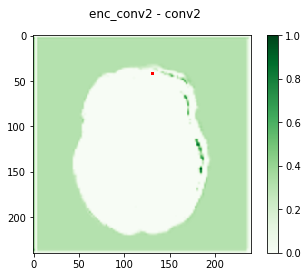
\includegraphics[width=\linewidth]{chapters/04_segmentation/images/grad_cam_05.png}
        \caption{b}
    \end{subfigure}
        \begin{subfigure}{.33\textwidth}
        \centering
        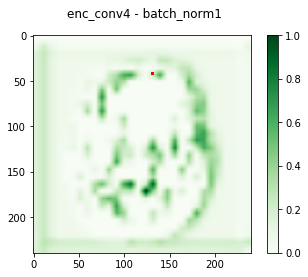
\includegraphics[width=\linewidth]{chapters/04_segmentation/images/grad_cam_14.png}
        \caption{b}
    \end{subfigure}
    \caption{Explanation text}
\end{figure}

\begin{figure}[H]
    \centering
    \begin{subfigure}{.33\textwidth}
        \centering
        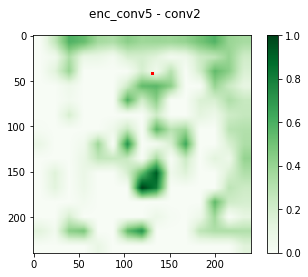
\includegraphics[width=\linewidth]{chapters/04_segmentation/images/grad_cam_17.png}
        \caption{ the text for a}
    \end{subfigure}%
    \begin{subfigure}{.33\textwidth}
        \centering
        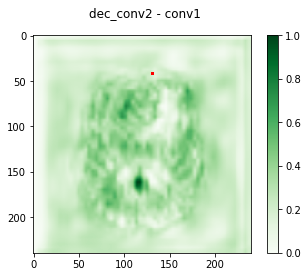
\includegraphics[width=\linewidth]{chapters/04_segmentation/images/grad_cam_24.png}
        \caption{b}
    \end{subfigure}
        \begin{subfigure}{.33\textwidth}
        \centering
        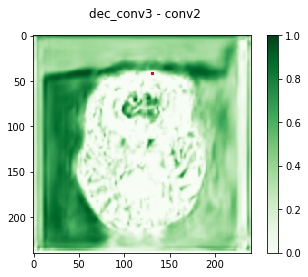
\includegraphics[width=\linewidth]{chapters/04_segmentation/images/grad_cam_29.png}
        \caption{b}
    \end{subfigure}
    \caption{Explanation text}
\end{figure}

\begin{figure}[H]
    \centering
    \begin{subfigure}{.33\textwidth}
        \centering
        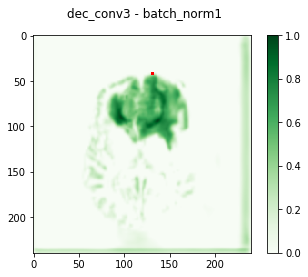
\includegraphics[width=\linewidth]{chapters/04_segmentation/images/grad_cam_30.png}
        \caption{ the text for a}
    \end{subfigure}%
    \begin{subfigure}{.33\textwidth}
        \centering
        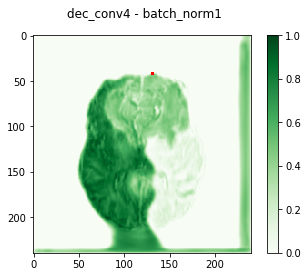
\includegraphics[width=\linewidth]{chapters/04_segmentation/images/grad_cam_34.png}
        \caption{b}
    \end{subfigure}
        \begin{subfigure}{.33\textwidth}
        \centering
        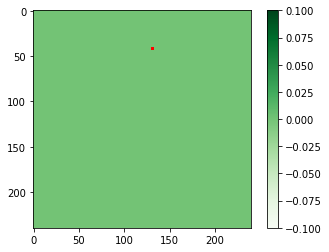
\includegraphics[width=\linewidth]{chapters/04_segmentation/images/grad_cam_36.png}
        \caption{b}
    \end{subfigure}
    \caption{Explanation text}
\end{figure}

\subsection{Discussion}
TODO

\subsection{Conclusion}
TODO

Because of these results, we decided to not modify Grad-CAM to work on multiple pixels and move to other methods.